\section{Methodology}
\lhead{\leftmark}
The equipment needed and procedures undertaken to carry out CNC Machining are described in the following sections. The experiment was done at ENW-04 (Machine Shop) at the JKUAT Workshops.
\subsection{Equipment}
\begin{enumerate}
\item CNC Machine ()
\item Workpiece design as specified by the manual
\item CNC Machine controller (Siemends Sinumerik 828D)
\item Workpiece - Aluminium block 
\end{enumerate}
\begin{figure}[h!]
	\centering
	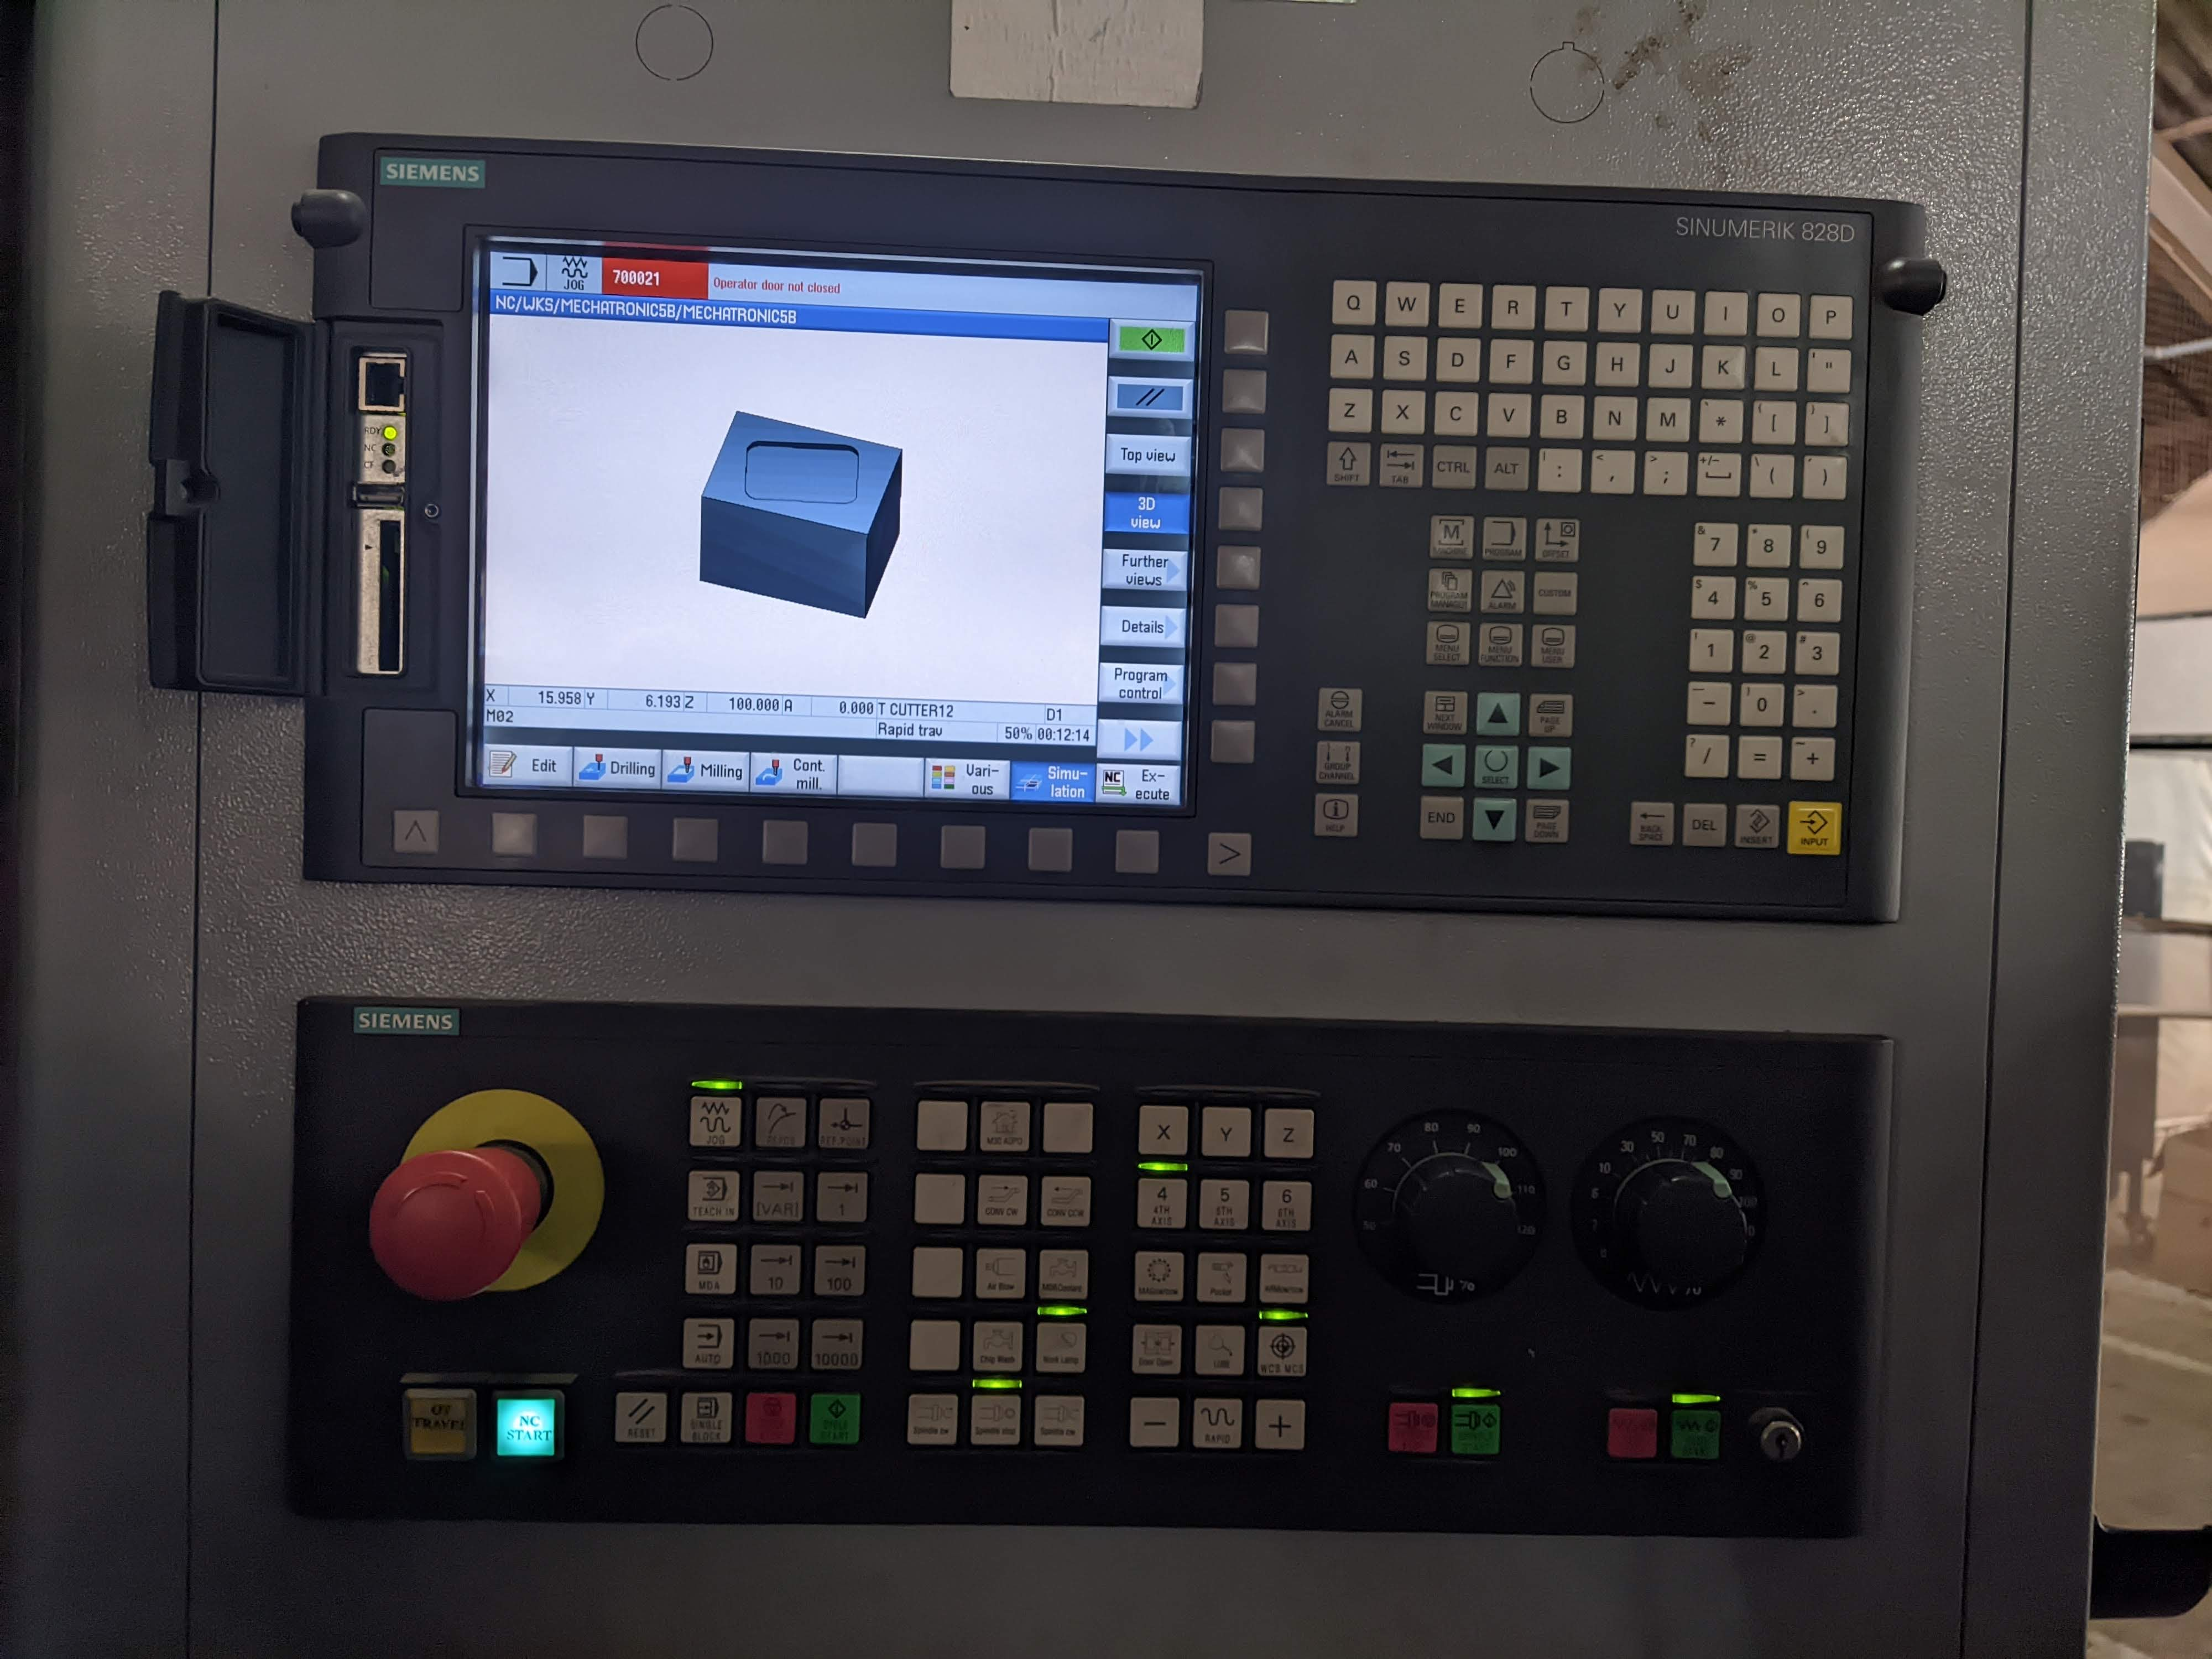
\includegraphics[width=0.7\linewidth]{Figures/machinecontroller}
	\caption[CNC Machine Controller]{CNC Machine Controller - Siemens SINUMERIK\textsuperscript\textregistered 828D} 
	\label{fig:cnccontroller}
\end{figure}
\subsection{Procedure}
Prior to beginning the machining operation, the machine has to be checked for the required items for its functionality, namely:
\begin{enumerate}
	\item Oil - This is necessary for lubrication and is contained in an oil tank at the back of the machine.
	\item Air - the pneumatic system is used by the tool change mechanism, and is supplied via high-pressure pipes and air ducts from an air compressor.
	\item Electricity - 3-$\phi$ electricity is required for the machine drives to move the various axes along.
\end{enumerate}
The shape to be created was analysed and the dimensions obtained. A toolpath was created using G codes to control the EDM Machine. The codes were programmed into the EDM Machine.\\
Once the program was loaded in the machine, the wire electrode was carefully placed at a small distance from the edge of the workpiece. The pump was then turned on and the dielectric fluid, in this case water, was used to fill the dielectric tank. Once the water level reached the trigger floaters, the machine was ready to begin the machining process, thus was turned on and the machining process done.\\
Once the machining process was completed, the tank was once again drained and the workpiece retrieved for examination.
\begin{figure}[h!]
	\centering
	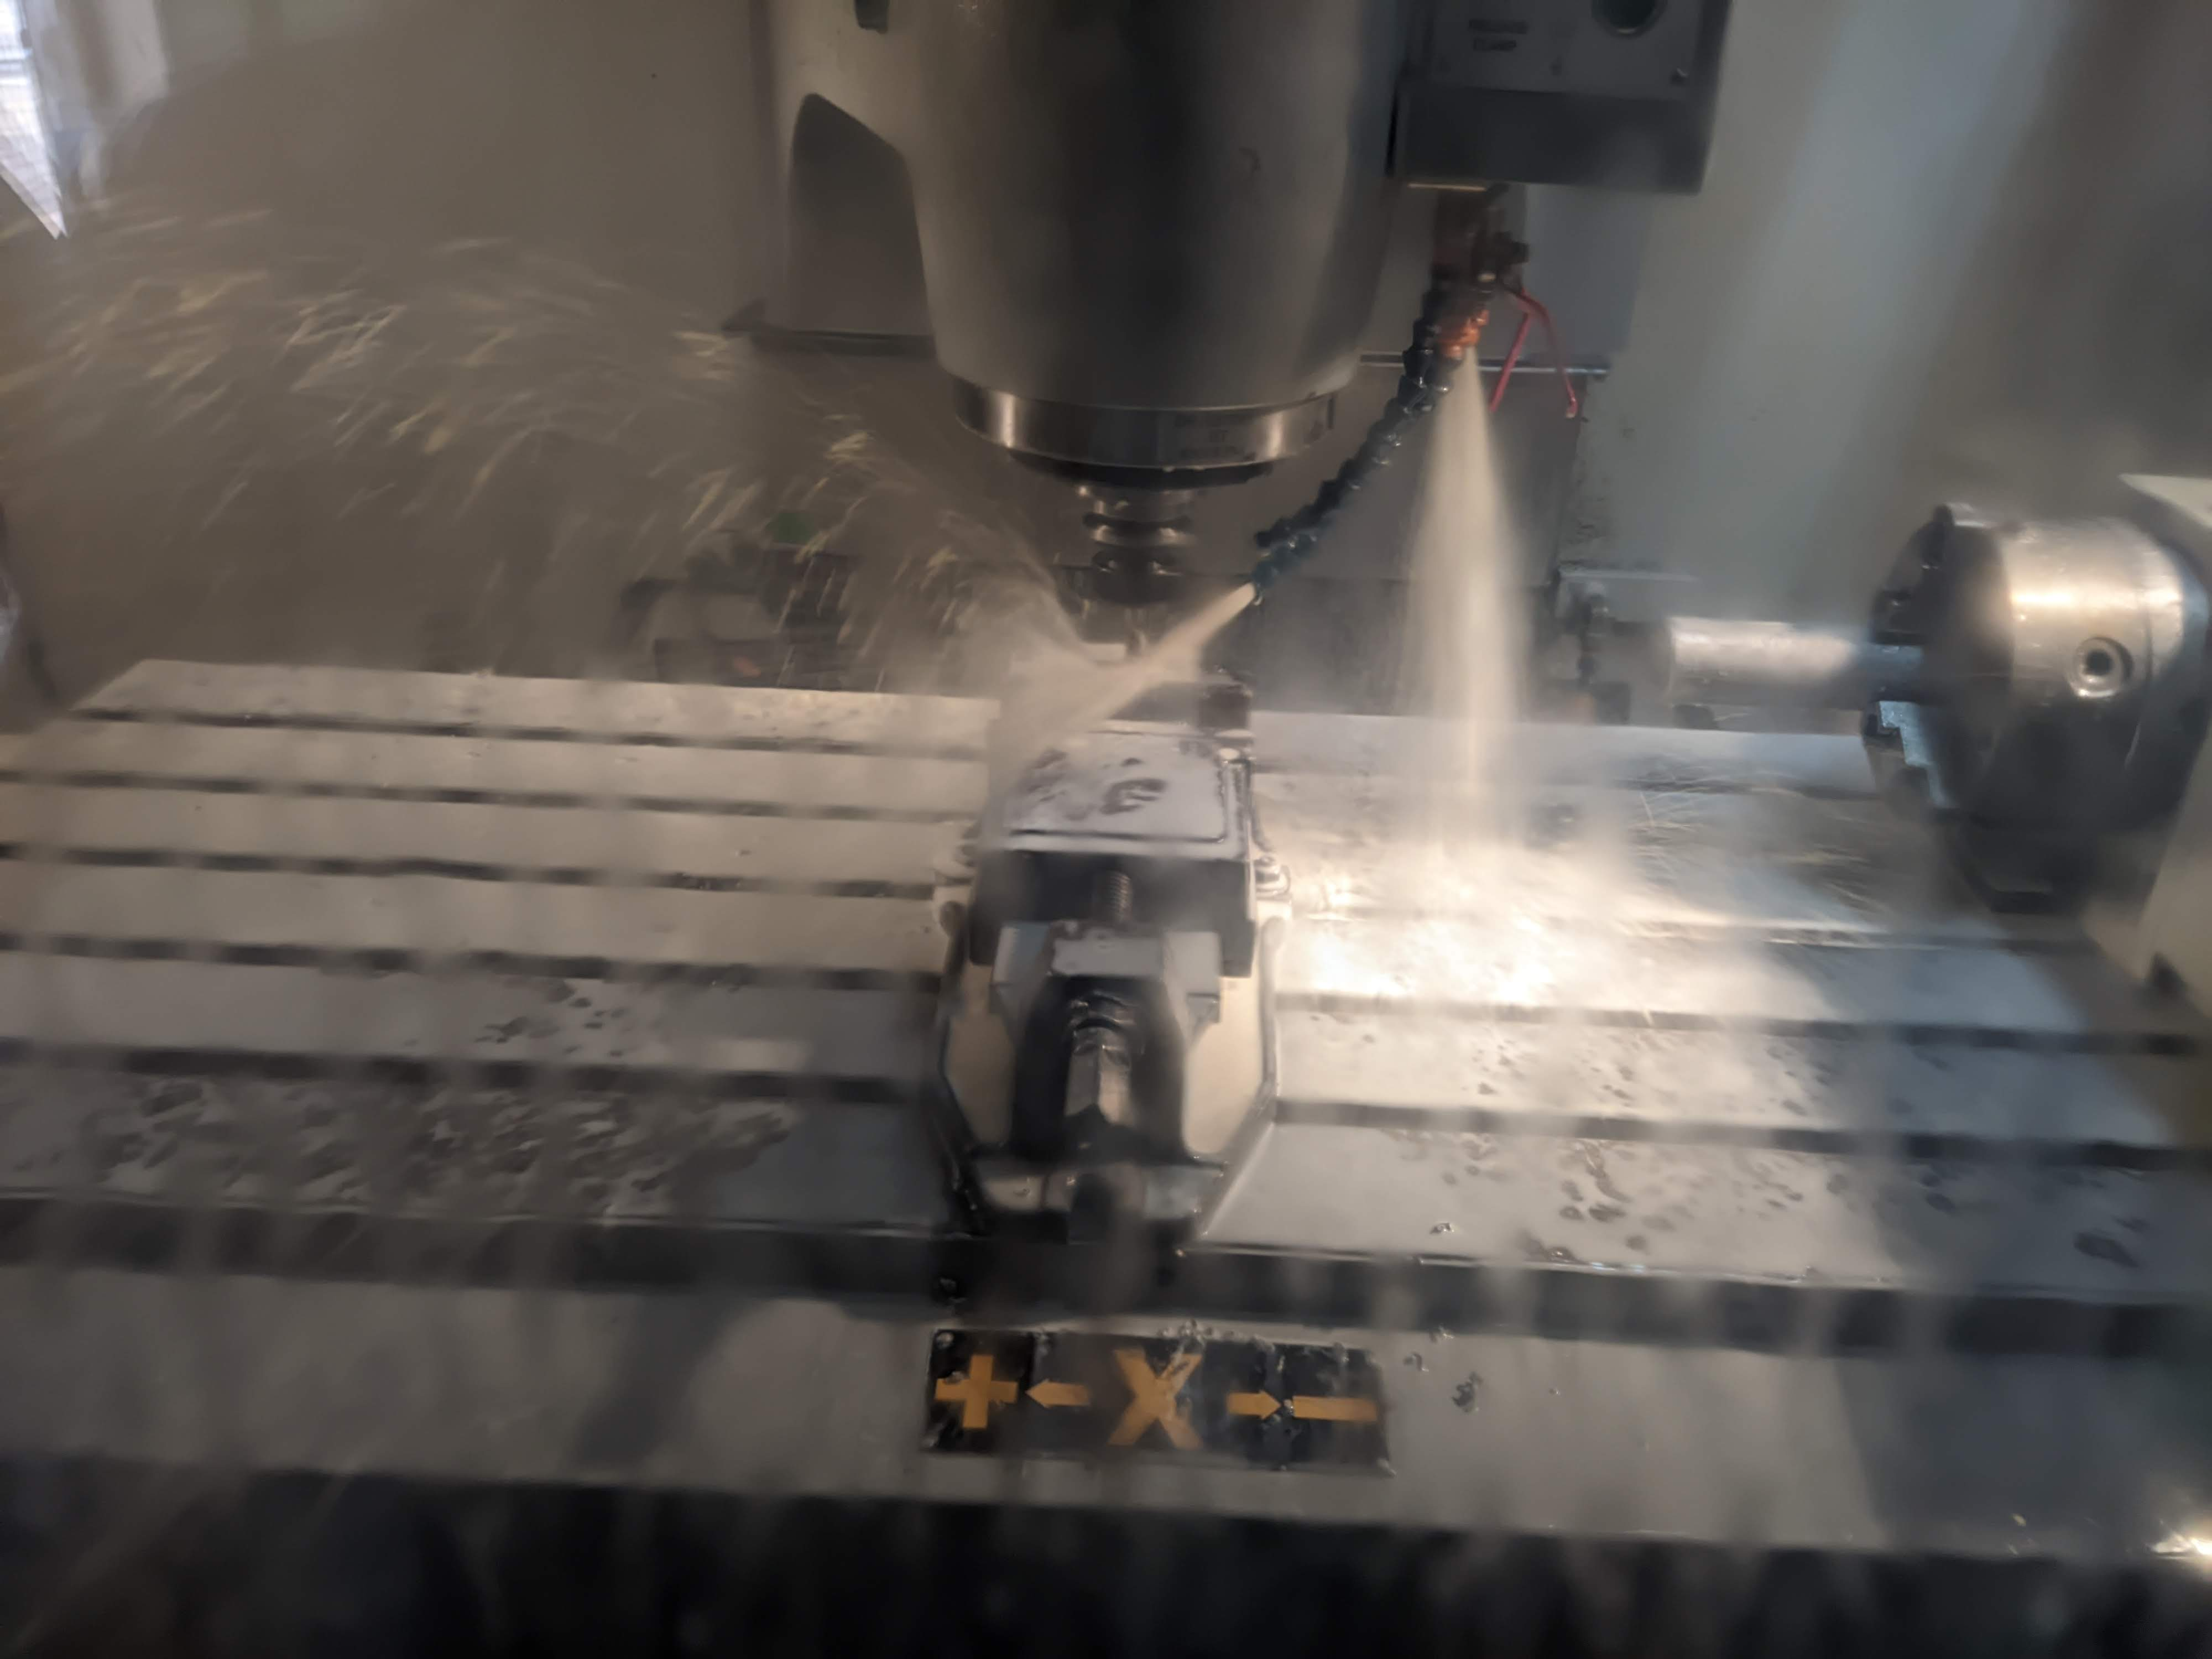
\includegraphics[width=0.7\linewidth]{Figures/machining}
	\caption[CNC Machining Process]{CNC Machining Process Underway}
	\label{fig:machining}
\end{figure}
\subsection{EDM Machining Program}
The program used to machine the workpiece was  handwritten and then transferred to the EDM Machine Controller. The program is as follows:
%\begin{verbatim}
%	G21
%	G92 X0.0 Y0.0
%	S1D1
%	G01 X7.0 Y0.0
%	G01 X0.0 Y-7.0
%	G01 X-7.0 Y0.0
%	G00 X0.0 Y0.0
%	M02
%\end{verbatim}